\documentclass[pscyr,nonums]{hedlab}
\usepackage[russian]{babel}
\usepackage[utf8]{inputenc}
\usepackage{graphicx}
\usepackage{listings}
\usepackage{subcaption}
\usepackage{wrapfig}

\labnum{2}
\labname{Введение в разработку WinPhone-приложений.}
\student{Голубев А.~В.}
\labdate{}

\begin{document}
    \makeheader
    \lstset{language=[Sharp]C, basicstyle=\tiny}

    \noindent\emph{Цель работы:} 
    \begin{enumerate}
        \item познакомится с инструментами разработки WinPhone-приложения
        \item разобрать структуру типичного WinPhone-приложения
        \item научиться запускать приложение на эмуляторе
    \end{enumerate}

    \noindent Калькулятор
    \begin{wrapfigure}{r}{0.3\textwidth} 
        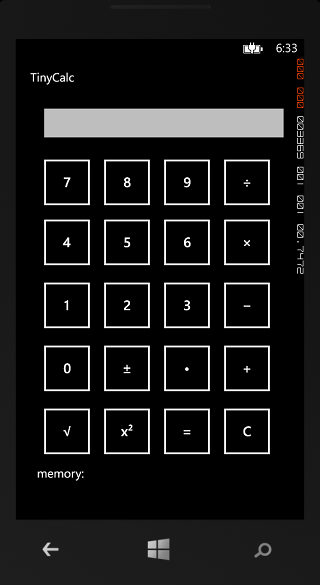
\includegraphics[width=.3\textwidth]{image}
    \end{wrapfigure}
    \lstinputlisting{code.cs}
\end{document}
